\documentclass{article}
\usepackage[margin=1in]{geometry}
\usepackage{amsmath}
\usepackage{amssymb}
\usepackage{amsthm}
\usepackage{bm}
\usepackage{hyperref}
\usepackage{graphicx}
\usepackage{caption}
\usepackage{listings}
\usepackage{xcolor}
\usepackage{float}
\usepackage{booktabs}
\usepackage{longtable}
\usepackage{multirow}
\usepackage{placeins}
\graphicspath{{figures/}}

% Code style
\lstdefinestyle{code}{
  basicstyle=\ttfamily\small,
  numbers=left,
  numberstyle=\tiny,
  numbersep=8pt,
  keywordstyle=\color{blue},
  commentstyle=\color{teal!70!black},
  stringstyle=\color{orange!70!black},
  showstringspaces=false,
  breaklines=true,
  frame=single,
  framerule=0.3pt,
  rulecolor=\color{black!15}
}
\lstset{style=code}

\title{Evaluation and Interpretability: Benchmarks, Dimensions, and Attribution Tooling}
\author{}
\date{\today}

\begin{document}
\maketitle

\section{Benchmarks: MMLU, GSM8K, BIG-Bench}
\subsection{Benchmark landscape}
Figure~\ref{fig:benchmark_landscape_en} maps MMLU, GSM8K, and BIG-Bench along a capability spectrum. Together they cover broad knowledge, multi-step reasoning, and long-tail evaluations (including safety and creativity).
\begin{figure}[H]
  \centering
  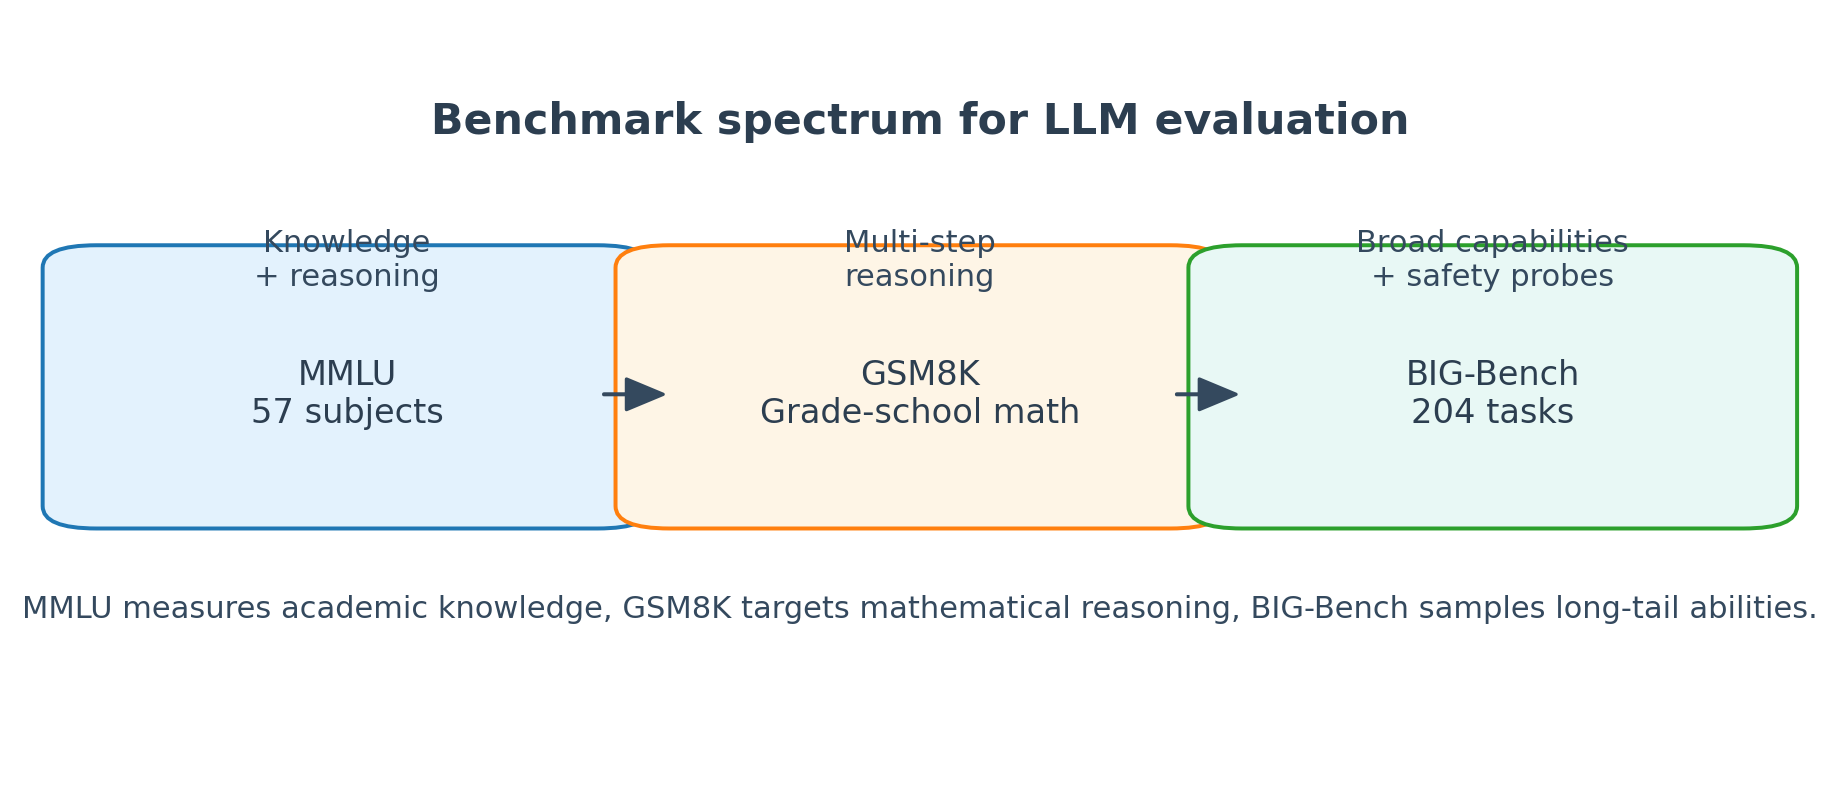
\includegraphics[width=0.9\textwidth]{benchmark_landscape.png}
  \caption{Benchmark spectrum across knowledge (MMLU), mathematical reasoning (GSM8K), and generalized capabilities (BIG-Bench).}
  \label{fig:benchmark_landscape_en}
\end{figure}

\subsection{MMLU}
\begin{itemize}
  \item 57 academic subjects with 15K multiple-choice questions spanning STEM, social sciences, humanities.
  \item Tests factual recall, contextual understanding, and out-of-domain transfer.
  \item Variants include translated versions, chain-of-thought prompting, and few-shot evaluation.
\end{itemize}

\subsection{GSM8K}
\begin{itemize}
  \item Focuses on grade-school math word problems requiring step-by-step reasoning.
  \item Chain-of-thought prompting and self-consistency sampling dramatically boost accuracy.
  \item Extensions involve harder math sets, program-aided solving, and verification loops.
\end{itemize}

\subsection{BIG-Bench}
\begin{itemize}
  \item 204 diverse tasks, including logic puzzles, ethics, multimodal reasoning, and adversarial challenges.
  \item BIG-Bench Hard isolates tasks humans solve easily but models find difficult—ideal for frontier evaluations.
  \item Supports crowd-sourced task contributions, enabling rapid growth of long-tail assessments.
\end{itemize}

\section{Evaluation Dimensions: Knowledge, Reasoning, Safety, Values}
\subsection{Dimension matrix}
\begin{longtable}{p{3cm}p{4cm}p{6cm}}
\toprule
Dimension & Representative benchmarks & Focus areas \\
\midrule
Knowledge & MMLU, TruthfulQA & Factual accuracy, specialized expertise, freshness \\
Reasoning & GSM8K, ARC-Challenge, MathBench & Multi-step deduction, symbolic manipulation, planning \\
Safety & RealToxicity, AdvBench, JailbreakBench & Harmful content detection, jailbreak resistance, policy compliance \\
Values alignment & Anthropic Helpful/Harmless, Constitutional AI evals & Moral alignment, cultural sensitivity, normative coherence \\
\bottomrule
\end{longtable}

\subsection{Evaluation workflow}
\begin{enumerate}
  \item Maintain a unified evaluation repository (static benchmarks + custom datasets) with standardized prompts.
  \item Integrate online telemetry (user feedback, refusal rates) to complement offline scores.
  \item Automate reporting: trend dashboards, anomaly detection, SLA alerts.
  \item Continuously red-team safety and alignment dimensions; refresh adversarial sets frequently.
\end{enumerate}

\subsection{Metrics and diagnostics}
\begin{itemize}
  \item Accuracy, macro/micro F1, exact match for classification and QA tasks.
  \item Chain analytics: reasoning length, error type taxonomy, tool usage counts.
  \item Safety metrics: refusal ratio, toxic incidence, recovery rate after unsafe prompt.
  \item Alignment metrics: sentiment ratio, cross-cultural consistency, human preference scores.
\end{itemize}

\section{Attention Visualization and Attribution Analysis}
\subsection{Interpretability pipeline}
Figure~\ref{fig:interpretability_pipeline_en} outlines the lifecycle from instrumenting inputs to deriving insights via attention probes and attribution scores.
\begin{figure}[H]
  \centering
  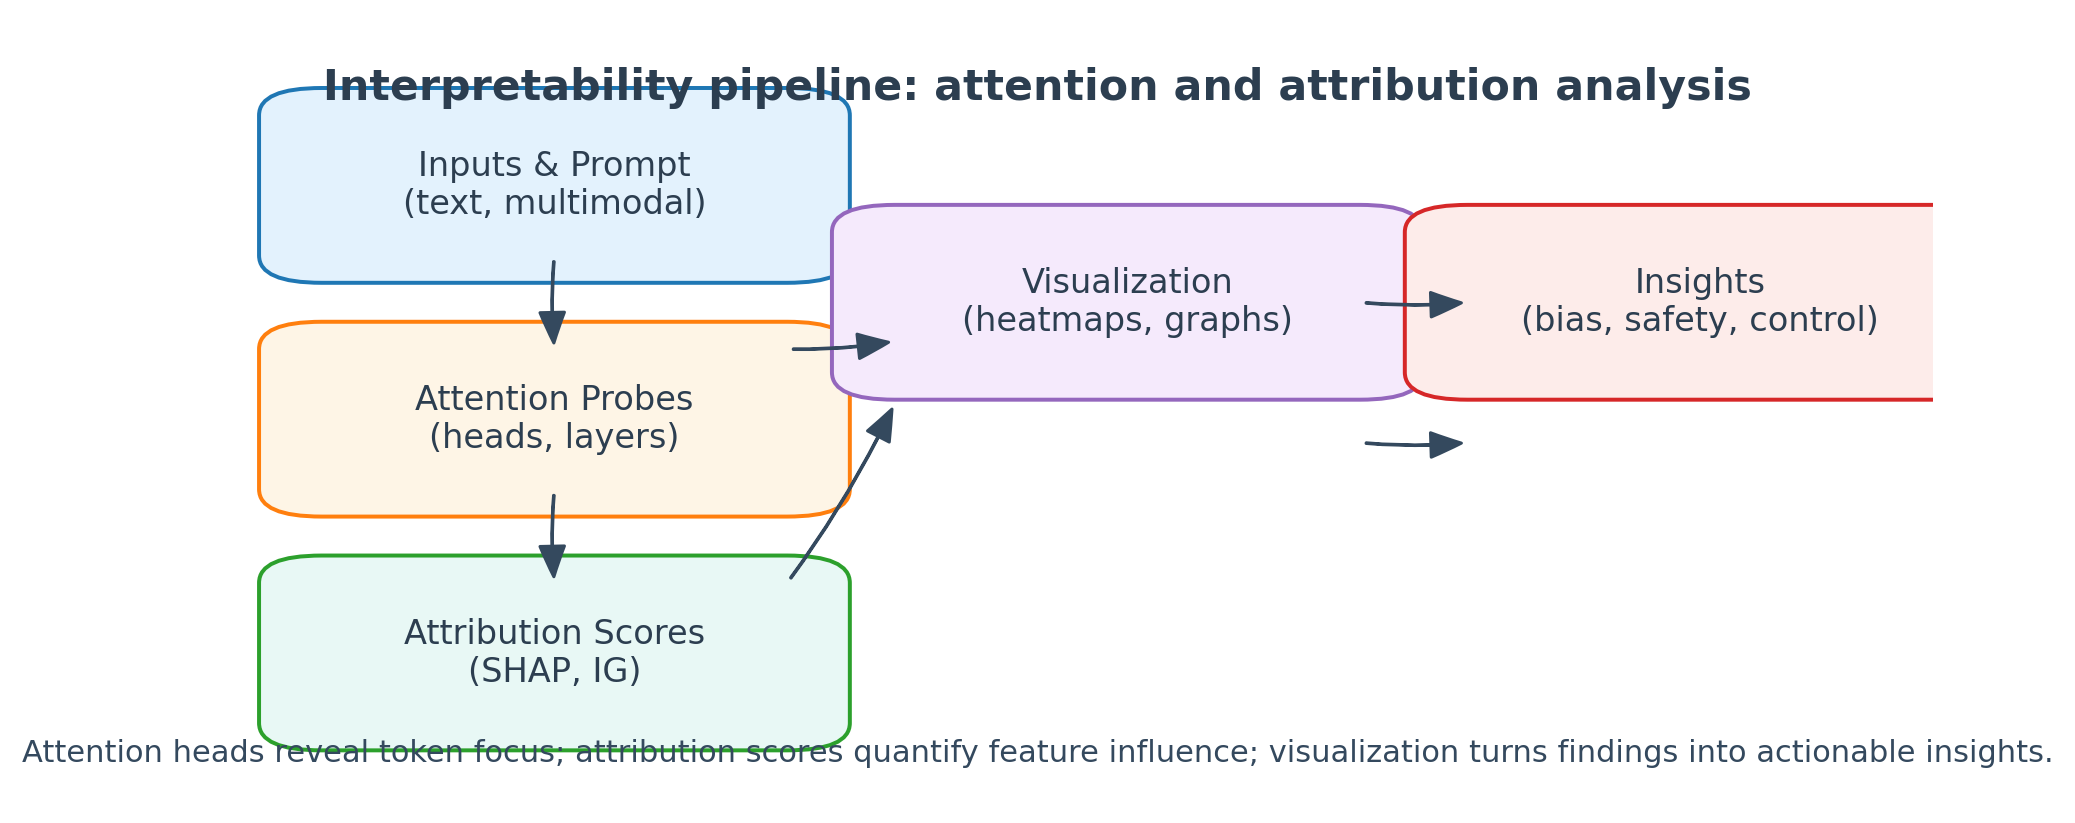
\includegraphics[width=0.9\textwidth]{interpretability_pipeline.png}
  \caption{Interpretability pipeline combining attention probing, attribution scoring, visualization, and insights.}
  \label{fig:interpretability_pipeline_en}
\end{figure}

\subsection{Attention probing}
\begin{itemize}
  \item \textbf{Attention rollout:} Multiplies attention matrices across layers to estimate token influence.
  \item \textbf{Attention flow:} Accounts for residuals/MLPs to better approximate information flow (Chefer et al.).
  \item \textbf{Head importance:} Gradient or masking-based head scoring reveals redundant attention heads for pruning.
\end{itemize}

\subsection{Attribution methods}
\begin{itemize}
  \item \textbf{Integrated Gradients (IG):} Computes path-integrated gradients from a baseline to quantify feature contribution.
  \item \textbf{SHAP:} Game-theoretic attribution adaptable to tabular, text, and multimodal inputs.
  \item \textbf{Layer-wise relevance propagation (LRP):} Propagates relevance through deep networks, capturing non-linear interactions.
\end{itemize}

\subsection{Example: IG with LLaMA}
\begin{lstlisting}[language=Python,caption={Integrated Gradients attribution for a LLaMA model}]
import torch
from transformers import AutoModelForCausalLM, AutoTokenizer
from captum.attr import IntegratedGradients

model_name = "meta-llama/Llama-2-7b-chat-hf"
tokenizer = AutoTokenizer.from_pretrained(model_name)
model = AutoModelForCausalLM.from_pretrained(model_name, torch_dtype=torch.float16).cuda()
model.eval()

prompt = "Explain the greenhouse effect."
inputs = tokenizer(prompt, return_tensors="pt").to(model.device)

def forward(inputs_ids, attention_mask):
    outputs = model(input_ids=inputs_ids, attention_mask=attention_mask)
    return outputs.logits[:, -1, :].max(dim=-1).values

ig = IntegratedGradients(forward)
baseline = torch.zeros_like(inputs["input_ids"])

attributions, _ = ig.attribute(
    inputs["input_ids"],
    baselines=baseline,
    additional_forward_args=(inputs["attention_mask"],),
    return_convergence_delta=True,
)

tokens = tokenizer.convert_ids_to_tokens(inputs["input_ids"][0])
for token, score in zip(tokens, attributions[0].sum(dim=-1).tolist()):
    print(f"{token}: {score:.4f}")
\end{lstlisting}

\subsection{Visualization techniques}
\begin{itemize}
  \item Token heatmaps overlay attribution scores on text; color intensity reveals focus.
  \item Attention graphs depict head-to-token relationships using networkx or graphviz.
  \item Interactive dashboards (Streamlit, Gradio) allow filtering samples, comparing models, and annotating anomalies.
\end{itemize}

\section*{Operational recommendations}
\begin{itemize}
  \item Align evaluation dimensions with product goals; combine static benchmarks and dynamic telemetry.
  \item Maintain reproducible evaluation pipelines with versioned datasets and code.
  \item Use interpretability findings to categorize failure modes (hallucination, bias, reasoning gaps) and feed results back into training.
  \item Perform red-team and gray-box audits before deployment; archive evaluations for compliance reviews.
\end{itemize}

\section*{Further reading}
\begin{itemize}
  \item Hendrycks et al. ``Measuring Massive Multitask Language Understanding.'' ICLR, 2021.
  \item Cobbe et al. ``Training Verifiers to Solve Math Word Problems.'' arXiv, 2021.
  \item Srivastava et al. ``Beyond the Imitation Game Benchmark (BIG-bench).'' arXiv, 2022.
  \item Chefer et al. ``Transformers Interpretability Beyond Attention Visualization.'' CVPR, 2021.
  \item Mukherjee et al. ``LLM Introspection: Improving Safety via Interpretability.'' arXiv, 2023.
\end{itemize}

\end{document}

